\whiteBGstarBegin
\setcounter{section}{0}
\section{Trắc nghiệm}
\begin{enumerate}[label=\bfseries Câu \arabic*:]
	
	
	\item \mkstar{1}
	
	\cauhoi
	{Chọn phát biểu đúng. Nhiễm điện do hưởng ứng xảy ra khi
		\begin{mcq}
			\item đưa một vật mang điện lại gần một vật dẫn điện đang trung hòa điện (đặt trên một giá cách điện).
			\item có electron dịch chuyển từ nguyên tử này sang nguyên tử khác, từ vật này sang vật khác.
			\item đưa một vật mang điện dương tiếp xúc với vật đang trung hòa điện.
			\item đưa một vật mang điện dương tiếp xúc với vật mang điện âm (đặt trên giá cách điện).
		\end{mcq}
		
	}
	\loigiai
	{	\textbf{Đáp án: A.}
		
		Nhiễm điện do hưởng ứng xảy ra khi đưa một vật mang điện lại gần vật dẫn điện đang trung hòa về điện.
	}
	\item \mkstar{1}
	
	\cauhoi
	{Chọn câu \textbf{sai}. Điện trường đều
		\begin{mcq}
			\item có cường độ như nhau tại mọi điểm.
			\item có đường sức là những đường song song cách đều nhau.
			\item xuất hiện giữa hai bản kim loại phẳng, song song và tích điện trái dấu.
			\item là điện trường tồn tại xung quanh điện tích điểm.
		\end{mcq}
		
	}
	\loigiai
	{	\textbf{Đáp án: D.}
		
		Điện trường đều là điện trường có cường độ như nhau tại mọi điểm, có đường sức là những đường thẳng song song cách đều nhau và xuất hiện giữa hai bản kim loại phẳng, song song và tích điện trái dấu.
	}
	\item \mkstar{1}
	
	\cauhoi
	{Phát biểu nào sau đây \textbf{không đúng}?
		\begin{mcq}
			\item Theo thuyết electron, một vật nhiễm điện dương là vật thiếu electron.
			\item Theo thuyết electron, một vật nhiễm điện âm là vật thừa electron.
			\item Theo thuyết electron, một vật nhiễm điện dương là vật đã nhận thêm các ion dương.
			\item Theo thuyết electron, một vật nhiễm điện âm là vật đã nhận thêm các electron.
		\end{mcq}
		
	}
	\loigiai
	{	\textbf{Đáp án: C.}
		
		Theo thuyết electron, một vật nhiễm điện dương là vật thiếu electron (mất electron), một vật nhiễm điện âm là vật thừa electron (nhận thêm electron).
	}
	\item \mkstar{1}
	
	\cauhoi
	{Trong các đại lượng vật lí sau, đại lượng nào là đại lượng vectơ?
		\begin{mcq}(2)
			\item Đường sức điện.
			\item Điện tích.
			\item Cường độ điện trường.
			\item Điện trường.
		\end{mcq}
		
	}
	\loigiai
	{	\textbf{Đáp án: C.}
		
		Cường độ điện trường là một đại lượng vectơ.
	}
	\item \mkstar{2}
	
	\cauhoi
	{Có hai điện tích điểm $q_1$ và $q_2$ đặt trong không khí, chúng hút nhau bằng một lực $F$. Khi đưa chúng vào trong dầu có hằng số điện môi $\varepsilon = 2$, vẫn giữ nguyên khoảng cách thì lực hút giữa chúng là
		\begin{mcq}(4)
			\item $F'=F$.
			\item $F'=2F$.
			\item $F'=F/2$.
			\item $F'=F/4$.
		\end{mcq}
		
	}
	\loigiai
	{	\textbf{Đáp án: C.}
		
		Lập tỉ lệ:
		$$\dfrac{F}{F'} = \dfrac{\varepsilon}{1} = 2 \Rightarrow F'=\dfrac{F}{2}.$$
	}
	\item \mkstar{2}
	
	\cauhoi
	{Khi một điện tích $q$ di chuyển trong một điện trường từ điểm A đến điểm B thì lực điện sinh công $\SI{4.5}{J}$. Nếu thế năng của $q$ tại A là $\SI{4.5}{J}$ thì thế năng tại B của nó là
		\begin{mcq}(4)
			\item $\SI{-4.5}{J}$.
			\item $\SI{-9}{J}$.
			\item $\SI{9}{J}$.
			\item $\SI{0}{J}$.
		\end{mcq}
		
	}
	\loigiai
	{	\textbf{Đáp án: D.}
		
	$$A_\text{AB} = W_\text A - W_\text B \Rightarrow W_\text B = \SI{0}{J}.$$
	}
	\item \mkstar{2}
	
	\cauhoi
	{Chọn câu đúng. Hai điện tích điểm đặt cách nhau một khoảng $r$. Dịch chuyển để khoảng cách giữa hai điện tích đó tăng lên 3 lần, nhưng vẫn giữ nguyên độ lớn điện tích của chúng. Khi đó lực tương tác giữa hai điện tích
		\begin{mcq}(2)
			\item tăng lên 3 lần.
			\item giảm đi 3 lần.
			\item tăng lên 9 lần.
			\item giảm đi 9 lần.
		\end{mcq}
		
	}
	\loigiai
	{	\textbf{Đáp án: D.}
		
		Lập tỉ số:
		$$\dfrac{F_1}{F_2} = \dfrac{3^2}{1} = 9 \Rightarrow F_2 = \dfrac{F_1}{9}.$$
	}
	\item \mkstar{2}
	
	\cauhoi
	{Chọn phát biểu đúng.
		\begin{mcq}
			\item Độ lớn của lực tương tác tĩnh điện giữa hai điện tích điểm tăng gấp 4 lần nếu khoảng cách giữa chúng tăng gấp đôi.
			\item Môi trường đặt hai điện tích điểm có hằng số điện môi càng lớn thì độ lớn của lực tương tác tĩnh điện giữa chúng càng lớn.
			\item Nếu độ lớn của một trong hai điện tích điểm tăng gấp đôi thì độ lớn lực tương tác tĩnh điện giữa chúng giảm đi một nửa.
			\item Độ lớn của lực tương tác tĩnh điện giữa hai điện tích điểm giảm đi 16 lần nếu khoảng cách giữa chúng tăng lên 4 lần.
		\end{mcq}
		
	}
	\loigiai
	{	\textbf{Đáp án: D.}
		
		Đáp án A sai vì lực tương tác tỉ lệ nghịch với khoảng cách $r$: $F$ tăng thì $r$ giảm;
		
		Đáp án B sai vì hằng số điện môi tỉ lệ nghịch với lực tương tác: $\varepsilon$ tăng thì $F$ giảm;
		
		Đáp án C sai vì lực tương tác tỉ lệ thuận với tích độ lớn của hai điện tích: độ lớn điện tích tăng thì $F$ tăng.
		.
	}
	\item \mkstar{2}
	
	\cauhoi
	{Một tụ điện có điện dung $\SI{5e-6}{F}$. Điện tích của tụ điện bằng $\SI{86}{\micro C}$. Hỏi hiệu điện thế trên hai bản tụ bằng bao nhiêu?
		\begin{mcq}(4)
			\item $U=\SI{27.2}{V}$.
			\item $U=\SI{37.2}{V}$.
			\item $U=\SI{47.2}{V}$.
			\item $U=\SI{17.2}{V}$.
		\end{mcq}
		
	}
	\loigiai
	{	\textbf{Đáp án: D.}
		
		Hiệu điện thế giữa hai bản tụ:
		$$U=\dfrac{Q}{C} = \SI{17.2}{V}.$$
	}
	\item \mkstar{2}
	
	\cauhoi
	{Có 4 vật A, B, C, D kích thước nhỏ, nhiễm điện. Biết rằng vật A hút vật B nhưng lại đẩy vật C. Vật C hút vật D. Khẳng định nào sau đây là \textbf{sai}?
		\begin{mcq}
			\item Điện tích của vật A và D cùng dấu.
			\item Điện tích của vật A và D trái dấu.
			\item Điện tích của vật B và D trái dấu.
			\item Điện tích của vật A và C cùng dấu.
		\end{mcq}
		
	}
	\loigiai
	{	\textbf{Đáp án: B.}
		
		Vật A hút vật B nên A trái dấu B;
		
		Vật A đẩy vật C nên A cùng dấu C;
		
		Vật C hút vật D nên C cùng dấu D.
		
		Suy ra A cùng dấu D, D khác dấu B.
	}
	\item \mkstar{2}
	
	\cauhoi
	{Tại một điểm có 2 cường độ điện trường thành phần vuông góc nhau và có độ lớn lần lượt là 3000 V/m và 4000 V/m. Độ lớn của cường độ điện trường tổng hợp là
		\begin{mcq}(4)
			\item 5000 V/m.
			\item 1000 V/m.
			\item 6000 V/m.
			\item 7000 V/m.
		\end{mcq}
		
	}
	\loigiai
	{	\textbf{Đáp án: A.}
		
		Với trường hợp hai vectơ cường độ điện trường thành phần vuông góc với nhau thì cường độ điện trường tổng hợp có độ lớn là
		$$E=\sqrt{E_1^2 + E_2^2} = \SI{5000}{V/m}.$$
	}
	\item \mkstar{3}
	
	\cauhoi
	{Một tụ điện không khí có điện dung 50 pF, khoảng cách giữa hai bản là 1 cm. Tính điện tích tối đa có thể tích cho tụ, biết rằng khi cường độ điện trường trong không khí lên đến $\SI{3e6}{V/m}$ thì không khí sẽ trở nên dẫn điện.
		\begin{mcq}(4)
			\item $\SI{15e4}{C}$.
			\item $\SI{15e-7}{C}$.
			\item $\SI{10e-7}{C}$.
			\item $\SI{3e-7}{C}$.
		\end{mcq}
		
	}
	\loigiai
	{	\textbf{Đáp án: B.}
		
		Điện tích tối đa trên một bản tụ là điện tích mà khi đó không khí vẫn còn là chất cách điện. Suy ra hiệu điện thế giữa hai bản tụ khi đó là
		$$U=Ed = \SI{3e4}{V}.$$
		
		Điện tích tối đa có thể tích cho tụ:
		$$Q=CU = \SI{15e-7}{C}.$$
	}
	\item \mkstar{3}
	
	\cauhoi
	{Cho hai điện tích $q_1=\SI{8e-8}{C}$, $q_2=\SI{2e-8}{C}$ lần lượt đặt tại hai điểm A và B cách nhau 10 cm trong chân không. Điểm M mà tại đó cường độ điện trường bằng 0 ở vị trí
		\begin{mcq}
			\item nằm trong khoảng AB, cách B là 10 cm.
			\item nằm trong khoảng AB, cách B là $\SI{3.3}{cm}$.
			\item nằm ngoài khoảng AB, cách A là 20 cm, cách B là 10 cm.
			\item nằm ngoài khoảng AB, cách A là 10 cm, cách B là 20 cm.
		\end{mcq}
		
	}
	\loigiai
	{	\textbf{Đáp án: B.}
		
		Để $\vec E = \vec E_\text{1M} + \vec E_\text{2M} = 0$ thì $\vec E_\text{1M} = -\vec E_\text{2M}$. Hệ quả: $\vec E_\text{1M}$ cùng phương, ngược chiều với $\vec E_\text{2M}$, còn về độ lớn thì $E_\text{1M} = E_\text{2M}$.
		
		Để $\vec E_\text{1M}$ cùng phương, ngược chiều với $\vec E_\text{2M}$ thì M phải nằm trong khoảng AB.
		
		Để $E_\text{1M} = E_\text{2M}$ thì $2\cdot \text{MB} = \text{AM}$. Suy ra $\text{MB} = \SI{3.3}{cm}$ và $\text{AM} = \SI{6.6}{cm}$.
		
		Vậy M nằm trong khoảng AB và cách B một khoảng $\SI{3.3}{cm}$.
	}
	\item \mkstar{3}
	
	\cauhoi
	{Trong không khí, người ta bố trí hai điện tích điểm có cùng độ lớn $\SI{1}{\micro C}$ nhưng trái dấu, cách nhau 2 m. Tại trung điểm của hai điện tích, cường độ điện trường là
		\begin{mcq}
			\item $\SI{18000}{V/m}$, hướng về điện tích dương.
			\item $\SI{18000}{V/m}$, hướng về điện tích âm.
			\item $\SI{0}{V/m}$.
			\item $\SI{18000}{V/m}$, hướng vuông góc với đoạn nối hai điện tích.
		\end{mcq}
		
	}
	\loigiai
	{	\textbf{Đáp án: B.}
		
		Biểu diễn vectơ cường độ điện trường thì thấy $\vec E = \vec E_1 + \vec E_2$ hướng về phía điện tích âm.
		\begin{center}
			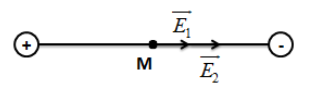
\includegraphics{../figs/VN11-2021-PH-TP011-1}
		\end{center}
	
	Độ lớn:
	$$E=E_1+E_2 = \SI{18000}{V/m}.$$
	}
	\item \mkstar{3}
	
	\cauhoi
	{Hai điện tích điểm $q_1=4q$ và $q_2=-q$ đặt tại hai điểm A, B cách nhau 9 cm trong chân không. Điểm M có cường độ điện trường bằng 0 cách B một khoảng
		\begin{mcq}(4)
			\item 27 cm.
			\item 9 cm.
			\item 18 cm.
			\item $\SI{4.5}{cm}$.
		\end{mcq}
		
	}
	\loigiai
	{	\textbf{Đáp án: B.}
		
	Do $q_1$ và $q_2$ trái dấu và $|q_1| > |q_2|$ nên vị trí cường độ điện trường tổng hợp bằng 0 nằm ngoài đoạn AB và ở phía B. Khi đó:
	$$E_1 = E_2 \Rightarrow k \dfrac{|4q|}{(r+9)^2} = k \dfrac{|-q|}{r^2} \Rightarrow r=\SI{9}{cm}.$$
	
	Điểm M có cường độ điẹn trường bằng 0 cách B một khoảng 9 cm.
	}
	\item \mkstar{3}
	
	\cauhoi
	{Một hạt bụi khối lượng $\SI{3.6e-15}{kg}$ nằm lơ lửng giữa hai tấm kim loại song song nằm ngang và nhiễm điện trái dấu. Điện tích của nó bằng $\SI{4.8e-18}{C}$. Tính độ lớn cường độ điện trường giữa hai tấm đó, lấy $g=\SI{10}{m/s^2}$.
		\begin{mcq}(4)
			\item $E=\SI{750}{V/m}$.
			\item $E=\SI{7500}{V/m}$.
			\item $E=\SI{75}{V/m}$.
			\item $E=\SI{1000}{V/m}$.
		\end{mcq}
		
	}
	\loigiai
	{	\textbf{Đáp án: B.}
		
		Để hạt bụi nằm cân bằng thì độ lớn lực điện $F$ bằng độ lớn trọng lực $P$:
		$$F=P \Rightarrow qE = mg \Rightarrow E = \dfrac{mg}{q} = \SI{7500}{V/m}.$$
	}
	\item \mkstar{3}
	
	\cauhoi
	{Một tụ điện phẳng được mắc vào hai cực của một nguồn điện có hiệu điện thế là $\SI{500}{V}$. Ngắt tụ điện ra khỏi nguồn rồi tăng khoảng cách giữa hai bản tụ lên 2 lần thì hiệu điện thế giữa hai bản của tụ điện đó
		\begin{mcq}(4)
			\item tăng 2 lần.
			\item tăng 4 lần.
			\item giảm 4 lần.
			\item giảm 2 lần.
		\end{mcq}
		
	}
	\loigiai
	{	\textbf{Đáp án: A.}
		
		Điện dung của tụ điện khi tăng khoagnr cách giữa hai bản lên 2 lần: $C'=\dfrac{C}{2}$.
		
		Mà $$Q=CU = C'U' \Rightarrow U'=\dfrac{C}{C'}U = 2U.$$
		
		Vậy $U$ tăng 2 lần.
	}
	\item \mkstar{3}
	
	\cauhoi
	{Đặt một điện tích thử $\SI{-1}{\micro C}$ tại một điểm thì nó chịu tác dụng của một lực điện $\SI{1}{mN}$ hướng từ trái qua phải. Cường độ điện trường tại vị trí đặt điện tích thử có độ lớn và chiều lần lượt là
		\begin{mcq}
			\item $\SI{1000}{V/m}$, hướng từ trái sang phải.
			\item $\SI{1}{V/m}$, hướng từ phải sang trái.
			\item $\SI{1}{V/m}$, hướng từ trái sang phải.
			\item $\SI{1000}{V/m}$, hướng từ phải sang trái.
		\end{mcq}
		
	}
	\loigiai
	{	\textbf{Đáp án: D.}
		
		Cường độ điện trường hướng từ phải sang trái (do $q<0$) và có độ lớn là
		$$E=\dfrac{F}{|q|} = \SI{1000}{V/m}.$$
	}
	\item \mkstar{3}
	
	\cauhoi
	{Ba điểm A, B, C tạo thành tam giác đều cạnh $a=\SI{100}{cm}$ nằm trong một điện trường đều $E=\SI{1000}{V/m}$, chiều từ B đến C. Hiệu điện thế $U_\text{CA}$ có giá trị bằng
		\begin{mcq}(4)
			\item $\SI{-500}{V}$.
			\item $\SI{-250}{V}$.
			\item $\SI{250}{V}$.
			\item $\SI{500}{V}$.
		\end{mcq}
		
	}
	\loigiai
	{	\textbf{Đáp án: A.}
		
		Hiệu điện thế $U_\text{CA}$:
		$$U_\text{CA} = Ea \cos 120^\circ = \SI{-500}{V}.$$
	}
	\item \mkstar{3}
	
	\cauhoi
	{Một electron bay từ điểm A đến điểm B trong điện trường, cho biết điện thế tại A là $V_\text{A} = \SI{150}{V}$, tại B là $V_\text{B} = \SI{50}{V}$. Độ biến thiên động năng của electron khi chuyển động từ A đến B là
		\begin{mcq}(4)
			\item $\SI{3.2e-17}{J}$.
			\item $\SI{-1.6e-17}{J}$.
			\item $\SI{1.6e-17}{J}$.
			\item $\SI{-3.2e-17}{J}$.
		\end{mcq}
		
	}
	\loigiai
	{	\textbf{Đáp án: B.}
		
		Độ biến thiên động năng bằng công của lực tĩnh điện:
		$$\Delta W_\text{đ} = A = qU_\text{AB} = q(V_\text{A} - V_\text{B}) = \SI{-1.6e-17}{J}.$$
	}
\end{enumerate}

\whiteBGstarEnd

\loigiai
{
	\begin{center}
		\textbf{BẢNG ĐÁP ÁN}
	\end{center}
	\begin{center}
		\begin{tabular}{|m{2.8em}|m{2.8em}|m{2.8em}|m{2.8em}|m{2.8em}|m{2.8em}|m{2.8em}|m{2.8em}|m{2.8em}|m{2.8em}|}
			\hline
			1.A  & 2.D  & 3.C  & 4.C  & 5.C  & 6.D  & 7.D  & 8.D  & 9.D  & 10.B  \\
			\hline
			11.A  & 12.B  & 13.B  & 14.B  & 15.B  & 16.B  & 17.A  & 18.D  & 19.A  & 20.B  \\
			\hline
		\end{tabular}
	\end{center}
}
\section{Tự luận}
\begin{enumerate}[label=\bfseries Câu \arabic*:]
	\item \mkstar{2}
	
	\cauhoi{
		Cho hai điện tích $q_1=\SI{2}{\micro C}$, $q_2=\SI{8}{\micro C}$ đặt tại hai điểm A và B trong chân không, với $\text{AB} = \SI{30}{cm}$. Xác định vị trí của điểm M để nếu đặt tại M một điện tích $q_0$ bất kì thì lực điện tổng hợp tác dụng lên $q_0$ bằng 0.
	}
	
	\loigiai{
		
		Vì $q_1$ và $q_2$ cùng dấu nên để lực điện tác dụng lên $q_0$ bằng 0 thì điểm đó phải nằm trên đoạn nối giữa $q_1$ và $q_2$. Khi đó:
		$$\vec F_{10} = - \vec F_{20}.$$
		
		Về độ lớn:
		$$F_{10} = F_{20} \Rightarrow k \dfrac{|q_1 q_0|}{r_1^2} = k \dfrac{|q_2 q_0|}{r_2^2}.$$
		
		Tìm được $r_1=\SI{10}{cm}$, $r_2=\SI{20}{cm}$.
	}
	
	\item \mkstar{2}
	
	\cauhoi{
		Tụ phẳng đặt trong không khí có điện dung $C=\SI{500}{pF}$, được tích điện đến hiệu điện thế $U=\SI{300}{V}$.
		\begin{enumerate}
			\item Tính điện tích $Q$ của tụ điện;
			\item Ngắt tụ điện ra khỏi nguồn. Nhúng tụ điện vào trong chất lỏng có $\varepsilon = 2$. Tính điện dung $C_1$, điện tích $Q_1$ và hiệu điện thế lúc đó;
			\item Vẫn nối tụ với nguồn. Nhúng tụ vào trong chất lỏng có $\varepsilon = 2$. Tính $C_2$, $Q_2$ và $U_2$ khi đó.
		\end{enumerate}
	}
	
	\loigiai{
		\begin{enumerate}
			\item Tính điện tích $Q$ của tụ điện;
			
			Điện tích của tụ:
			$$Q=CU = \SI{15e-8}{C}.$$
			
			\item Ngắt tụ điện ra khỏi nguồn. Nhúng tụ điện vào trong chất lỏng có $\varepsilon = 2$. Tính điện dung $C_1$, điện tích $Q_1$ và hiệu điện thế lúc đó;
			
			Khi ngắt tụ ra khỏi nguồn thì $Q$ không đổi nên điện tích của tụ lúc này là
			$$Q_1=Q=\SI{15e-8}{C}.$$
			
			Mà khi đó điện dung của tụ là
			$$C_1=2C = \SI{e-9}{F}.$$
			
			Vậy hiệu điện thế giữa hai bản tụ là
			$$U_1 = \dfrac{Q_1}{C_1} = \SI{150}{V}.$$
			
			\item Vẫn nối tụ với nguồn. Nhúng tụ vào trong chất lỏng có $\varepsilon = 2$. Tính $C_2$, $Q_2$ và $U_2$ khi đó.
			
			Khi vẫn nối tụ vào nguồn thì hiệu điện thế không đổi, khi đó hiệu điện thế giữa hai bản tụ là
			$$U_2 = U = \SI{300}{V}.$$
			
			Điện dung của tụ:
			$$C_2=2C = \SI{e-9}{F}.$$
			
			Điện tích của tụ:
			$$Q_2=C_2U_2 = \SI{3e-7}{C}.$$
		\end{enumerate}
		
	}
	\item \mkstar{2}
	
	\cauhoi{
		Đặt bốn điện tích âm có cùng độ lớn $q$ tại bốn đỉnh của một hình vuông ABCD cạnh $a$. Xác định cường độ điện trường tổng hợp tại giao điểm hai đường chéo của hình vuông.
	}
	
	\loigiai{
		Cường độ điện trường tại tâm O của hình vuông:
		$$\vec E_\text{O} = \vec E_\text{A} + \vec E_\text{B} + \vec E_\text{C} + \vec E_\text{D}.$$
		
		Độ lớn của các cường độ điện trường thành phần:
		$$E_\text{A} = E_\text{B} = E_\text{C} = E_\text{D} = k \dfrac{|q|}{\text{OA}^2}.$$
		
		Dễ thấy $\vec E_\text{AC} = \vec E_\text{A} + \vec E_\text{C} = 0$ và $\vec E_\text{BD} = \vec E_\text{B} + \vec E_\text{D} = 0$. Vậy cường độ điện trường tổng hợp tại O là
		$$\vec E_\text{O} = \vec E_\text{AC} + \vec E_\text{BD} = 0.$$
		
	}
	\item \mkstar{3}
	
	\cauhoi{
		Ba điểm A, B, C là ba đỉnh của một tam giác vuông tại A trong điện trường đều, cường độ $E=\SI{1000}{V/m}$. Đường sức điện trường song song với AC, chiều từ A đến C. Biết $\text{AC} = \SI{8}{cm}$, $\text{AB} = \SI{6}{cm}$.
		\begin{enumerate}
			\item Tính hiệu điện thế giữa các điểm A và B, A và C, B và C;
			\item Tính công của lực điện để dịch chuyển một electron từ điểm B đến điểm C;
			\item Một electron chuyển động không vận tốc đầu, xuất phát tại A, xác định vận tốc của electron đó khi nó di chuyển tới điểm C của tam giác đã cho.
		\end{enumerate}
	}
	
	\loigiai{
		\begin{enumerate}
			\item Tính hiệu điện thế giữa các điểm A và B, A và C, B và C;
			
			Vì điểm A và B nằm trên cùng một mặt đẳng thế nên $U_\text{AB} = 0$.
			
			Hiệu điện thế giữa A và C là
			$$U_\text{AC} = E \cdot \text{AC} = \SI{80}{V}.$$
			
			Hiệu điện thế giữa B và C là
			$$U_\text{BC} = E \cdot \text{BC} = \SI{100}{V}.$$
			\item Tính công của lực điện để dịch chuyển một electron từ điểm B đến điểm C;
			
			Công của lực điện:
			$$A=|e| \cdot U_\text{BC} = \SI{12.8e-8}{J}.$$
			
			\item Một electron chuyển động không vận tốc đầu, xuất phát tại A, xác định vận tốc của electron đó khi nó di chuyển tới điểm C của tam giác đã cho.
			
			Độ biến thiên động năng bằng công của lực điện:
			$$A_\text{AC} = W_\text{đ C} - W_\text{đ A} \Rightarrow v_\text{C} = \sqrt{\dfrac{2A_\text{AC}}{m}} = \SI{5.3e6}{m/s}.$$
		\end{enumerate}
		
	}
\end{enumerate}